\section{Overview}
\label{s:oview}

This section gives an overview of the definition of integer errors
and the analysis architecture.

\subsection{Integer Security}
\label{s:goal}

\sys assumes two's complement~\cite[\chapterautorefname~4.2.1]{intel:vol1},
a de facto standard integer representation on modern architectures.
An $n$-bit unsigned integer is in the range $0$ to $2^n-1$, while
an $n$-bit signed integer is in the range $-2^{n-1}$ to $2^{n-1}-1$,
with the most significant bit indicating the sign.  If not particularly
indicated, $x$ and $y$ below are $n$-bit integers.  A subscript $s$
or $u$ may be pinned to an operation to specify it operates on
signed or unsigned integers.

\sys adopts the CERT C secure coding standard for integer
operations~\cite[\chapterautorefname~5]{seacord:secure-c} as a basis
and considers operations that violate the coding standard as integer
errors.  They cover a set of integer-based vulnerabilities, sometimes
referred as arithmetic overflow (underflow, wraparound), division-by-zero,
oversized shift, and signedness bugs in the literature.  We will
summarize them below.

\paragraph{Addition \& subtraction \& multiplication.}
Such an operation may lead to an integer error if the result of the
corresponding arbitrary-precision mathematical operation falls out
of the predefined range.  For example, $\cc{maxnum}\times_u 16$
causes an integer error if $\cc{maxnum} = \cc{0xf0000000}$, because
the mathematical product $\cc{0xf0000000} \times 16 = 2^{32}\times
3\times 5$ is out of the range of $32$-bit unsigned integers ($0$
to $2^{32} - 1$).

\paragraph{Division.}
A division operation causes an integer error if the divisor is 0.
Additionally, signed division $x\ /_s\ y$ may lead to an integer
error if $x = -2^{n-1}$ and $y = -1$, because the mathematical
result $2^{n-1}$ is not in the range of $n$-bit signed integers
($-2^{n-1}$ to $2^{n-1}-1$).

\paragraph{Shift.}
The bitwise shifts $x \shl y$ and $x \shr y$ are considered as
integer errors if $y \geq_u n$, which is undefined according to the
C standard.  For example, $(1 \shl 32)$ may yield 0 (e.g., on x86)
or 1 (e.g., on PowerPC) for 32-bit integers, depending on the
underlying architecture.

\paragraph{Conversion.}
If $x$ is converted from integer type $s$ to $t$, the conversion
may lead to an integer error if the value of $x$ does not fall into
the range of $t$.  For example, in \autoref{f:ext4} the call to
\cc{ext4_split_extent} returns a signed int, which will be negative
on error.  However, the value is converted to an unsigned integer,
leading to a meaningless comparison that is always false.

\paraend

It is worth noting that with the secure integer standard two
functionally equivalent operations may have different error constraints.
It is assumed that developers have chosen the appropriate operations
to match their intention.  For example, $\cc{maxnum}\times_u 16$
may be erroneous if \cc{maxnum} is large, while $\cc{maxnum} \shl
4$ is considered always secure.  Any compiler optimization that
performs such code transformations would destroy the semantics.
Besides, decent C compilers may completely optimize away invalid
integer error checks like $(x + 1) < x$ for signed integer
$x$~\cite{gcc:signed-overflow,us-cert:gcc}, unless a special compile
option \cc{-fwrapv} or \cc{-fno-strict-overflow} is given.  Therefore,
\sys should work on unoptimized code.

\begin{figure}
\centering
\begin{Verbatim}[commandchars=\\\{\}]
\PY{k}{static} \PY{k+kt}{int} \PY{n}{ext4\PYZus{}split\PYZus{}extent}\PY{p}{(}\PY{p}{.}\PY{p}{.}\PY{p}{.}\PY{p}{)}\PY{p}{;}

\PY{k}{static} \PY{k+kt}{int} \PY{n+nf}{ext4\PYZus{}ext\PYZus{}convert\PYZus{}to\PYZus{}initialized}\PY{p}{(}\PY{p}{.}\PY{p}{.}\PY{p}{.}\PY{p}{)}
\PY{p}{\PYZob{}}
	\PY{k+kt}{unsigned} \PY{k+kt}{int} \PY{n}{allocated}\PY{p}{;}
	\PY{k+kt}{int} \PY{n}{err} \PY{o}{=} \PY{l+m+mi}{0}\PY{p}{;}
	\PY{p}{.}\PY{p}{.}\PY{p}{.}
	\PY{n}{allocated} \PY{o}{=} \PY{n}{ext4\PYZus{}split\PYZus{}extent}\PY{p}{(}\PY{p}{.}\PY{p}{.}\PY{p}{.}\PY{p}{)}\PY{p}{;}
	\PY{k}{if} \PY{p}{(}\PY{n}{allocated} \PY{o}{<} \PY{l+m+mi}{0}\PY{p}{)}
		\PY{n}{err} \PY{o}{=} \PY{n}{allocated}\PY{p}{;}
	\PY{k}{return} \PY{n}{err} \PY{o}{?} \PY{n}{err} \PY{o}{:} \PY{n}{allocated}\PY{p}{;}
\PY{p}{\PYZcb{}}
\end{Verbatim}

\caption{A signedness bug in the ext4 filesystem of the Linux kernel.
Since \texttt{allocated} is declared as unsigned int, the test
$(\texttt{allocated} < 0)$ will always be false, which breaks the
error handling.}
\label{f:ext4}
\end{figure}

\subsection{A Strawman Analysis}

\sys is implemented as a set of compiler passes in the
LLVM~\cite{lattner:llvm} framework, as shown in \autoref{f:flow}.
For each integer operation it first performs symbolic analysis to
compute the error constraint and the corresponding path constraint
(ignore range constraint for now).  These passes work on the
intermediate representation (IR), which is compiled from source
code with all optimizations turned off.

As for $\cc{maxnum} \times_u 16$ in \autoref{f:bridge}, \sys computes
its error constraint as:
\begin{equation*}
\cc{maxnum} >_u (2^{32} - 1) / 16.
\end{equation*}
Since the multiplication is always reachable without any branches
in that function, the corresponding path constraint is simply true.

\sys then feeds the logical AND of the two constraints into a
constraint solver~\cite{boolector}.  The solver computes a possible
input, e.g., $\cc{maxnum} = \cc{0xf0000000}$.

Now let's consider the patched code that correctly limits \cc{maxnum}
to 256, shown as below (\cc{maxnum} is
numbered~\cite[\chapterautorefname~8.11]{whale} for clarification
purpose).
\begin{Verbatim}[commandchars=\\\{\}]
\PY{n}{maxnum0} \PY{o}{=} \PY{p}{.}\PY{p}{.}\PY{p}{.}\PY{p}{;} \PY{c+cm}{/* read from userspace */} 
\PY{k}{if} \PY{p}{(}\PY{n}{maxnum0} \PY{o}{>} \PY{n}{PAGE\PYZus{}SIZE} \PY{o}{/} \PY{k}{sizeof}\PY{p}{(}\PY{k}{struct} \PY{n}{\PYZus{}\PYZus{}fdb\PYZus{}entry}\PY{p}{)}\PY{p}{)}
    \PY{n}{maxnum1} \PY{o}{=} \PY{n}{PAGE\PYZus{}SIZE} \PY{o}{/} \PY{k}{sizeof}\PY{p}{(}\PY{k}{struct} \PY{n}{\PYZus{}\PYZus{}fdb\PYZus{}entry}\PY{p}{)}\PY{p}{;}
\PY{k}{else}
    \PY{n}{maxnum1} \PY{o}{=} \PY{n}{maxnum}\PY{p}{;}
\PY{n}{size} \PY{o}{=} \PY{n}{maxnum1} \PY{o}{*} \PY{k}{sizeof}\PY{p}{(}\PY{k}{struct} \PY{n}{\PYZus{}\PYZus{}fdb\PYZus{}entry}\PY{p}{)}\PY{p}{;}
\PY{n}{buf} \PY{o}{=} \PY{n}{kmalloc}\PY{p}{(}\PY{n}{size}\PY{p}{,} \PY{n}{GFP\PYZus{}USER}\PY{p}{)}\PY{p}{;}
\PY{p}{.}\PY{p}{.}\PY{p}{.}
\end{Verbatim}

The error constraint of the multiplication remains unchanged.
\begin{equation*}
\cc{maxnum}_1 >_u (2^{32} - 1) / 16.
\end{equation*}
The corresponding path constraint is that \cc{maxnum} is reset to 256
if it is larger than 256, or remains the old value otherwise.
\begin{align*}
& ((\cc{maxnum}_0 >_u 256) \land (\cc{maxnum}_1 = 256)) \\
\lor
& (\neg (\cc{maxnum}_0 >_u 256) \land (\cc{maxnum}_1 = \cc{maxnum}_0)).
\end{align*}
Again \sys takes the logical AND of the two constraints to the
constraint solver, which will conclude that these constraints can
never be satisfied.  This means that the integer error has been
fixed.

\begin{figure}
\centering
\resizebox{0.9\linewidth}{!}{
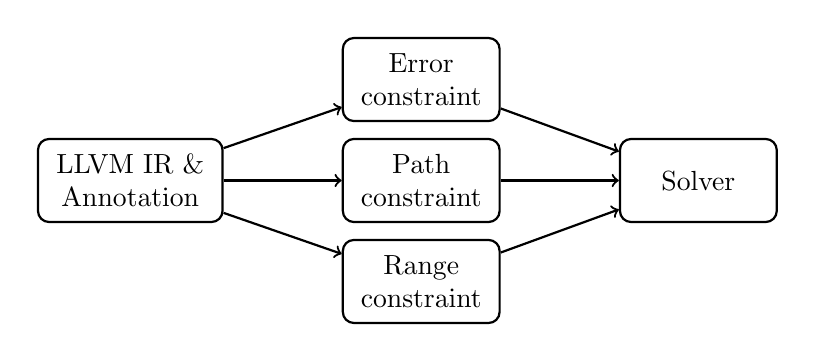
\begin{tikzpicture}[
	block/.style={
		rectangle, rounded corners,
		draw=black, thick,
		text width=5em, minimum height=3em, text centered
	},
	line/.style={draw, thick, ->},
	]
	\matrix[row sep=2mm, column sep=15mm] {
		& \node [block] (ec) {Error constraint}; & \\
		\node [block, text width=6em] (ir) {LLVM IR \& Annotation};
		& \node [block] (pc) {Path constraint};
		& \node [block] (sol) {Solver}; \\
		& \node [block] (rc) {Range constraint}; & \\
	};

	\path [line] (ir) -- (ec);
	\path [line] (ir) -- (pc);
	\path [line] (ir) -- (rc);
	\path [line] (ec) -- (sol);
	\path [line] (pc) -- (sol);
	\path [line] (rc) -- (sol);
\end{tikzpicture}

}
\caption{\sys's workflow.}
\label{f:flow}
\end{figure}

\if 0

\subsection{Challenges}
\label{s:chal}

There are several challenges that face \sys when applying the
secure integer standard described in \autoref{s:goal} to real-world
systems code.

\subsubsection{Benign Integer Errors}

While violating the secure integer standard, some commonly-used C
idioms will not cause any defects.  We recognize them as follows.

\paragraph{Partial violation.}
Take $(x +_u 1) -_u 2$ with $x \geq_u 1$ for an example.  The
expression would be considered as an integer error since the first
part $(x +_u 1)$ may be insecure, though the whole expression is
equivalent to $x -_u 1$ and will not cause any integer error.
Another example is that signed and unsigned integers are often used
interchangeably in C code.  In a conversion like \cc{(int)((unsigned)x)}
for a signed $x <_s 0$, the part \cc{(unsigned)x} may violate the
secure integer standard while the whole expression does not.  \sys
should avoid to warn against such ``partial'' violations.

\paragraph{Error-before-use.}
An integer error check may come after the overflowed computation,
but before any use of the result.  In that case, the overflowed
computation is benign.  Below is such an example.
\begin{Verbatim}[commandchars=\\\{\},codes={\catcode`\$=3\catcode`\^=7\catcode`\_=8}]
\PY{k+kt}{unsigned} \PY{n}{size} \PY{o}{=} \PY{n}{x} \PY{o}{*} \PY{n}{y}\PY{p}{;}
\PY{k}{if} \PY{p}{(}\PY{n}{x} \PY{o}{\PYZgt{}} \PY{n}{UINT\PYZus{}MAX} \PY{o}{/} \PY{n}{y}\PY{p}{)}
    \PY{k}{return} \PY{o}{-}\PY{l+m+mi}{1}\PY{p}{;}
\PY{p}{.}\PY{p}{.}\PY{p}{.} \PY{o}{=} \PY{n}{malloc}\PY{p}{(}\PY{n}{size}\PY{p}{)}\PY{p}{;}
\end{Verbatim}

Even the multiplication $x \times_u y$ overflows, the product
\cc{size} is not used before the check.  \sys will move the integer
operation $x \times_u y$ down to the latest possible point, i.e.,
right after the \cc{if} branch and before the \cc{malloc} call, so
as to avoid warning against the multiplication.

\paragraph{Overflowed checking idiom.}
It is commonly seen in practice to use an overflowed result to do
the integer error check for $x +_u y$:
\begin{align}
x +_u y <_u x.
\end{align}
This is equivalent to a ``sane'' check
$\cc{UINT_MAX} - x >_u y$.
\sys should recognize such integer error checking idioms and avoid
to warn against them.

Note that using overflowed result to check multiplication is trickier.
In general $x \times_u y <_u x$ is not a valid integer error check
but a bug.  A correct way would be $(x \times_u y) /_u y \neq x$
or a sane check, $\cc{UINT_MAX} /_u x > y$.

\subsubsection{Constraint Solving Performance}

Although \sys uses a highly-optimized constraint solver,
constraints generated unwisely would still hurt its performance,
sometimes even making it run forever.

\paragraph{Bounded constraint size.}
It is not a good idea to naively analyze and generate constraints
interprocedurally, for example,  across the whole Linux kernel.
The size of the path constraint would grow exponentially, which is
unnecessary and hard to solve.  To achieve scalability, \sys should
choose an appropriate program granularity.

\sys also needs to handle complex program constructs such as loops
and pointer arithmetic appropriately.  The generated constraints
should be able to catch common integer errors while being solvable
in a reasonable amount of time.

\paragraph{Idioms for faster solving.}
We notice that some operations like division would significantly
slow down the constraint solver~\cite{brummayer:perf}, most of which
are used in integer error checks like $\cc{UINT_MAX} /_u x > y$.
\sys should recognize these idioms and generate constraints that
are easier to solve.

\fi
